\documentclass[12pt,border=1pt]{standalone}
\usepackage[T1]{fontenc}
\IfFileExists{newtxtext.sty}{\usepackage{newtxtext,newtxmath}}{\usepackage{mathptmx}}
\usepackage{amsmath,amssymb}
\usepackage[table]{xcolor}
\usepackage{tikz}
\usetikzlibrary{arrows.meta,positioning,fit,calc,decorations.pathreplacing}
\tikzset{blk/.style={draw=black!55,rounded corners=2pt,align=center,font=\footnotesize,inner sep=4pt,minimum height=1.05cm},
         nn/.style={blk,fill=orange!12,draw=orange!70!black},
         lat/.style={blk,fill=blue!8,draw=blue!60!black},
         io/.style={blk,fill=black!3},
         arr/.style={-{Stealth[length=2.2mm]},thick,draw=black!65}}
\definecolor{capblue}{RGB}{47,84,150}
\definecolor{linkblue}{RGB}{17,85,204}
\definecolor{ganttA}{RGB}{11,90,110}
\definecolor{ganttB}{RGB}{20,150,160}
\definecolor{rowhl}{RGB}{253,236,224}
\definecolor{rowhl2}{RGB}{224,244,238}
\begin{document}
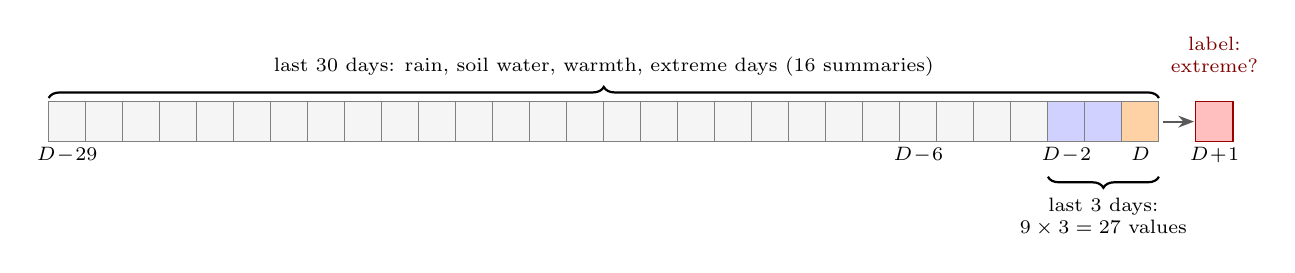
\begin{tikzpicture}[x=0.47cm,y=0.5cm,
  dbox/.style={draw=black!50,fill=#1,minimum height=0.5cm,minimum width=0.47cm,inner sep=0},
  ar/.style={-{Stealth[length=2mm]},thick,draw=black!65}]
\foreach \i in {0,...,29} { \node[dbox=black!4] at (\i,0) {}; }
\foreach \i in {27,28} { \node[dbox=blue!18] at (\i,0) {}; }
\node[dbox=orange!35] at (29,0) {};
\node[dbox=red!25,draw=red!60!black] at (31,0) {};
\node[font=\scriptsize,below] at (0,-0.4) {$D\!-\!29$};
\node[font=\scriptsize,below] at (23,-0.4) {$D\!-\!6$};
\node[font=\scriptsize,below] at (27,-0.4) {$D\!-\!2$};
\node[font=\scriptsize,below] at (29,-0.4) {$D$};
\node[font=\scriptsize,below] at (31,-0.4) {$D\!+\!1$};
\draw[decorate,decoration={brace,amplitude=4pt},thick] (-0.5,0.6) -- (29.5,0.6) node[midway,above=4pt,font=\scriptsize]{last 30 days: rain, soil water, warmth, extreme days (16 summaries)};
\draw[decorate,decoration={brace,amplitude=4pt,mirror},thick] (26.5,-1.4) -- (29.5,-1.4) node[midway,below=4pt,font=\scriptsize,align=center]{last 3 days:\\$9\times3=27$ values};
\node[font=\scriptsize,align=center,red!50!black] at (31,1.7) {label:\\extreme?};
\draw[ar] (29.6,0) -- (30.45,0);
\end{tikzpicture}
\end{document}
